%=====================================================================================================================
\section{Models, preregistered tests, deviations and withdrawn claims}\label{app:prereg}
\begin{table}[h]
\centering\scriptsize
\caption{Configurations. Wan-based cache models generate 832$\times$480 at 16\,fps in chunks of 3 latent frames
(0.75\,s); window and sink sizes are in latent frames.}
\label{tab:models}
\begin{tabular}{@{}p{3.6cm}p{4.6cm}p{1.2cm}p{4.4cm}@{}}
\toprule
Configuration & Base; training & Steps & Context of the opening \\
\midrule
Self Forcing DMD, SiD, SiD v2, GAN~\cite{selfforcing,dmd,sid} & Wan2.1-1.3B; self-rollout on 5-s clips & 4 & window 21; sink 0/1/3/6, original or re-rotated positions \\
Self Forcing 10\,s & Wan2.1-1.3B; self-rollout on 10-s clips & 4 & window 21, sink 3 \\
CausVid~\cite{causvid} & Wan2.1-1.3B; teacher-forced DMD & 3 & window 21, sink 0/3 \\
LongLive~\cite{longlive} & Wan2.1-1.3B; long-rollout tuning & 4 & window 12, sink 0/3 \\
Rolling Forcing~\cite{rollingforcing} & Wan2.1-1.3B; rolling joint denoising & 5 & anchor block + 21 \\
SkyReels-V2-DF~\cite{skyreels} & Wan2.1-1.3B architecture; diffusion forcing; 544p, 24\,fps & 30 + CFG & 17 (or 5) re-denoised overlapping frames \\
Matrix-Game-2.0~\cite{matrixgame2} & Wan2.1-1.3B architecture, no text; actions; 352$\times$640, 25\,fps & 3 & first latent frame only, window 6, no sink; CLIP image embedding \\
FramePack-F1 / I2V~\cite{framepack} & HunyuanVideo 13B; 480p, 30\,fps & 25 & clean prefix in every section; SigLIP image embedding \\
MAGI-1 4.5B-distill~\cite{magi} & own architecture (chunk-wise autoregressive diffusion transformer); 432$\times$768, 24\,fps, chunks of 1\,s & 64, pipelined & released: window of 4 earlier chunks, no sink; or full history \\
\bottomrule
\end{tabular}
\end{table}

% Every preregistered primary test, in order of freezing. Estimates are differences in the preregistered unit;
% intervals are 95% (Wald for studies 1-2 as preregistered, bootstrap otherwise); p is Holm-adjusted within the study.
\begin{table}[h]
\centering\scriptsize
\caption{All preregistered primary tests and their outcomes. Units: $D$, $K$ drift metrics; $|\Delta L|$ in \Lstar{};
$\alpha$ persistence. Arms: G generic prompt, M VLM caption of the opening, C calibrated lighting plus caption, ttc
content-aware correction.}
\label{tab:primary}
\begin{tabular}{@{}llllll@{}}
\toprule
Study & Test & Model & Estimate [95\% CI] & $p_{\text{Holm}}$ & Outcome \\
\midrule
1 Context & sink 3 vs none, $D$ & SF & $-7.56$ \ci{-8.32}{-6.81} & $<0.001$ & supported \\
  & sink 3 vs none, $K$ & SF & $-0.90$ \ci{-1.04}{-0.76} & $<0.001$ & supported \\
  & window $\times$ sink, $D$ & SF & $+5.71$ \ci{4.21}{7.22} & $<0.001$ & supported \\
  & window $\times$ sink, $K$ & SF & $+0.67$ \ci{0.38}{0.95} & $<0.001$ & supported \\
2 Correction & ttc $\beta{=}1$, $D$ & SF & $-1.48$ \ci{-1.76}{-1.19} & $<10^{-23}$ & supported \\
  & ttc $\beta{=}1.5$, $D$ & SF & $-1.78$ \ci{-2.11}{-1.45} & $<10^{-24}$ & supported \\
3 Caption & M $-$ G, $|\Delta L|$ & SF & $-1.21$ \ci{-3.09}{0.36} & 0.58 & not supported \\
  & M+ttc $-$ M, $|\Delta L|$ & SF & $-1.00$ \ci{-1.89}{-0.12} & 0.14 & not supported \\
  & M $-$ G, $|\Delta L|$ & LL & $-0.19$ \ci{-2.00}{1.63} & 1.0 & not supported \\
  & M+ttc $-$ M, $|\Delta L|$ & LL & $-0.36$ \ci{-1.48}{0.75} & 1.0 & not supported \\
4 Calibrated & C $-$ M, $|\Delta L|$ & SF & $-1.24$ \ci{-2.54}{0.12} & 0.25 & not supported \\
  & C $-$ G, $|\Delta L|$ & SF & $-2.45$ \ci{-4.08}{-1.04} & 0.013 & supported \\
  & C $-$ M, $|\Delta L|$ & LL & $-1.15$ \ci{-2.59}{0.29} & 0.26 & not supported \\
  & C $-$ G, $|\Delta L|$ & LL & $-1.34$ \ci{-3.19}{0.55} & 0.26 & not supported \\
5 Calibrated (LL scale) & C $-$ M, $|\Delta L|$ & LL & $-1.36$ \ci{-3.06}{0.32} & 0.26 & not supported \\
  & C $-$ G, $|\Delta L|$ & LL & $-1.55$ \ci{-3.50}{0.39} & 0.26 & not supported \\
6 Relaxation & no sink $-$ sink, $\alpha_L$ (31\,s) & SF & $-0.06$ \ci{-0.17}{0.05} & 0.34 & not supported \\
  & no sink $-$ sink, $\alpha_L$ (31\,s) & LL & $-0.17$ \ci{-0.28}{-0.06} & 0.013 & supported \\
  & ttc $-$ none, $\alpha_L$ (31\,s) & SF & $+0.12$ \ci{0.05}{0.20} & 0.013 & supported \\
  & no sink $-$ sink, $\alpha_b$ (31\,s) & SF & $-0.26$ \ci{-0.34}{-0.18} & $<0.001$ & supported \\
7 Sink at 60\,s & sink $-$ no sink, $\alpha_L$ & SF & $+0.55$ \ci{0.45}{0.65} & $<10^{-9}$ & supported \\
  & sink $-$ no sink, $\alpha_L$ & CausVid & $+0.19$ \ci{0.14}{0.24} & $<10^{-6}$ & supported \\
8 Overlap & 5 $-$ 17 frames, $\alpha_L$ (20\,s) & SkyReels & $-0.24$ \ci{-0.40}{-0.09} & 0.014 & supported \\
%NEWROWS
\bottomrule
\end{tabular}
\end{table}


\paragraph{Deviations from the preregistrations.}
\begin{itemize}
\item \emph{Study 1} was frozen before analysis but after generation of its main videos had started, and its arms were
not pinned to one GPU architecture: 62\% of its nominal seed pairs ran on different architectures. Its preregistered
Wald intervals are reported; the prompt-cluster bootstrap interval for the main contrast is wider (\ci{-10.45}{-5.39}
for $D$) but leads to the same conclusion.
\item \emph{Study 3:} a preempted job resumed on another GPU type and split four LongLive openings across
architectures. We regenerated the affected arms on the original architecture; conclusions are unchanged.
\item \emph{Study 6:} the ODE-initialised Self Forcing student was replaced by SiD v2 before generation (it collapses to
blur after the opening). GPU pinning was replaced by an architecture guard that regenerates a task's outputs when a
resumed job lands on another architecture; paired arms of each preregistered contrast always share a task. Exploratory
configurations (sink 1; correction on LongLive and CausVid) were added after freezing but before any data, from
separate task lists, so their contrasts with the preregistered arms are not guaranteed to share an architecture.
Prompt-only reference rollouts were renamed after generation; no analysis code changed.
\item \emph{Study 7} reuses the 24 scenes of study 6, including the 6 whose 120-s curves motivated it. Restricted to the
18 other scenes, the sink effect is $+0.53$ \ci{0.42}{0.63} (Self Forcing) and $+0.18$ \ci{0.13}{0.24} (CausVid).
\item \emph{Studies 10 and 11} were run on two non-preemptible 4-GPU jobs and A40-only array tasks instead of the
preregistered all-queue arrays, because no large GPU was free on the shared queue; all their videos ran on A40 GPUs, so
pairing is unaffected. The other studies ran as preregistered.
\end{itemize}

\paragraph{Withdrawn or revised claims.} During the project we withdrew four claims after checks: that MUSIQ rewards
collapsed videos (it is merely insensitive); that the sink stabilises the default (trend difference $+0.5$
\ci{-2.4}{3.5}); that the model follows its context by 76\% (true only for artificial shifts); and that early dynamics
forecast the final brightness. The recursion's predicted Self Forcing plateau of 0.25--0.54 was missed (0.58 at 60\,s in study 7).

%=====================================================================================================================
\section{Drift metrics for prompt-only rollouts}\label{app:metrics}
For rollouts without a held opening, drift is measured against 10 (Self Forcing) or 5 (LongLive) fresh 5-s generations
of the same prompt. $D$ is the per-frame Mahalanobis distance of (Lab means, saturation, log sharpness) from the fresh
frames' distribution, and $K$ the mean cosine distance of a frame's DINOv2 feature to its 5 nearest fresh-frame
features, normalised by the fresh clips' own value; both are averaged over seconds 29--31. Transitions kept is the
median over held-out transition prompts of the corrected over the uncorrected first-to-last brightness change; values
above 1 mean the correction amplified the change.

%=====================================================================================================================
\section{Robustness}\label{app:robust}
\begin{figure}[h]
\centering
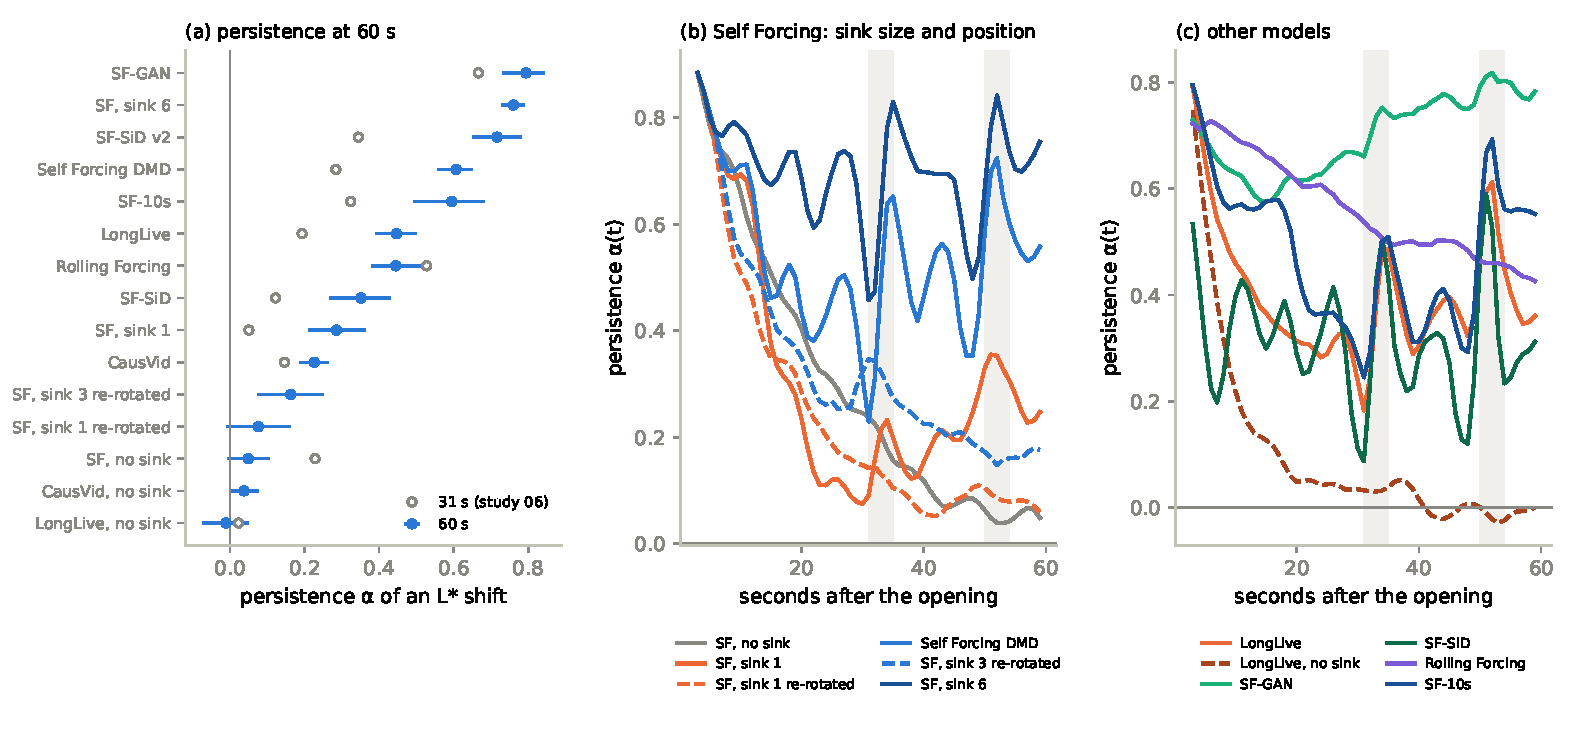
\includegraphics[width=\linewidth]{fig_atlas.pdf}
\caption{Persistence at 60\,s (study 10; CausVid from study 7). (a) $\alpha$ of an \Lstar{} shift with
scene-bootstrap 95\% CIs; hollow markers: 31\,s (study 6). (b) Self Forcing with sinks of 0, 1, 3 and 6 latent frames,
at their original positions or re-rotated to sit just before the window (dashed). (c) Other models. Curves: 1-s windows,
3-s moving average; shaded: 31--35\,s and 50--54\,s, where sinks of three or more frames at their original positions
produce bursts. The 60-s endpoint window, [50, 60)\,s, overlaps the second burst; Appendix~\ref{app:robust} reports a
burst-free window.}
\label{fig:atlas}
\end{figure}

\begin{figure}[h]
\centering
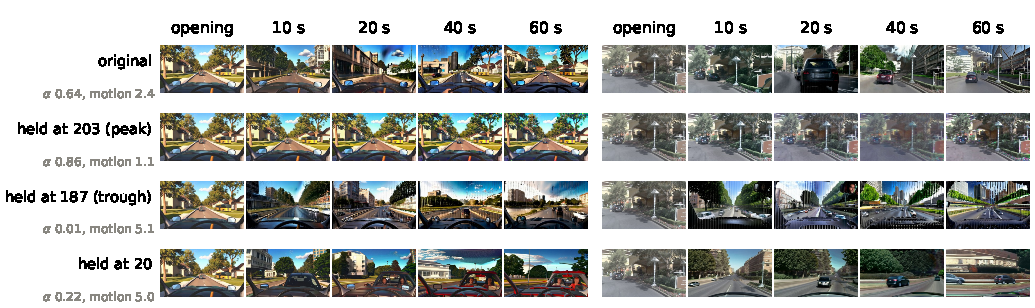
\includegraphics[width=\linewidth]{fig_s25frames.pdf}
\caption{Frames of two scenes (+16~\Lstar{} opening) continued by Self Forcing with a three-frame sink at its original
positions and held at query--sink distances 203 (a probe peak), 187 (the trough before it) and 20 (next to the window),
study 25. Held at the peak, the video stays on its opening; at the trough it leaves the opening within seconds, with
streak artefacts. Left: persistence $\alpha$ and mean frame-to-frame change (grey levels) over 50--60\,s, 24 scenes.}
\label{fig:s25frames}
\end{figure}

\begin{figure}[h]
\centering
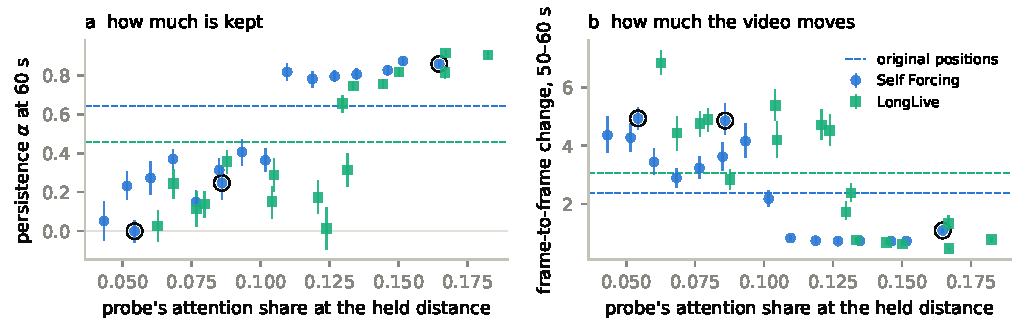
\includegraphics[width=\linewidth]{fig_held.pdf}
\caption{The sink held at one query--sink distance, 60-s videos, 24 scenes (study 27; circled: the three distances of
study 25). (a) Persistence $\alpha$ and (b) mean frame-to-frame change over 50--60\,s against the probe's attention
share at that distance, with scene-bootstrap 95\% CIs. Dashed: the sink at its original positions. Above a share of
about 0.105 every distance freezes the video on its opening; below it the video moves and persistence rises with the
share, more noisily.}
\label{fig:held}
\end{figure}

\begin{figure}[h]
\centering
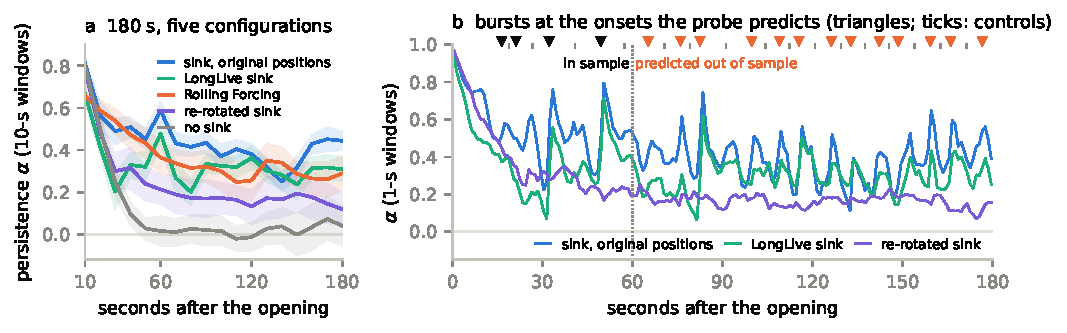
\includegraphics[width=\linewidth]{fig_long.pdf}
\caption{The 180-s horizon (studies 24 and 26; 24 scenes, Self Forcing unless named). (a) Persistence over 10-s
windows with scene-bootstrap 95\% CIs. An opening that stays in the context keeps a share to 180\,s; without a sink
it is forgotten by 50\,s. (b) Scene-mean 1-s curves. Triangles: burst onsets of the probe's major peaks for a sink at
its original positions; the four before 60\,s were seen when the probe was made, the 13 after 60\,s were
preregistered predictions (study 26). Ticks: control onsets midway between them. The re-rotated sink does not burst.}
\label{fig:long}
\end{figure}

\begin{table}[h]
\centering\scriptsize
\caption{Persistence over the same window, 15--20\,s after the opening, for every model (exploratory; scene-bootstrap
95\% CIs; Matrix-Game: scenes without a black second before 20\,s).}
\label{tab:matched}
\begin{tabular}{@{}lccc@{}}
\toprule
Configuration & $\alpha$ & 95\% CI & scenes \\
\midrule
SkyReels-V2-DF, 17 overlap frames & 1.01 & [0.89, 1.15] & 12 \\
FramePack-I2V, anti-drifting sampler & 0.86 & [0.79, 0.92] & 12 \\
SkyReels-V2-DF, 5 overlap frames & 0.77 & [0.64, 0.90] & 12 \\
Self Forcing DMD, sink 6 & 0.72 & [0.65, 0.78] & 24 \\
FramePack-F1, both routes & 0.68 & [0.56, 0.78] & 12 \\
Rolling Forcing & 0.64 & [0.60, 0.67] & 24 \\
Self Forcing GAN & 0.61 & [0.54, 0.67] & 24 \\
Self Forcing 10-s & 0.54 & [0.46, 0.63] & 24 \\
FramePack-F1, context prefix only & 0.53 & [0.31, 0.76] & 12 \\
Self Forcing DMD, sink 3 & 0.49 & [0.44, 0.53] & 24 \\
Self Forcing DMD, no sink & 0.44 & [0.38, 0.51] & 24 \\
Self Forcing DMD, sink 3 re-rotated & 0.38 & [0.28, 0.46] & 24 \\
Matrix-Game-2.0, both routes & 0.37 & [0.22, 0.52] & 17 \\
Self Forcing SiD & 0.34 & [0.24, 0.46] & 24 \\
LongLive, sink 3 & 0.33 & [0.25, 0.40] & 24 \\
Self Forcing DMD, sink 1 re-rotated & 0.33 & [0.25, 0.41] & 24 \\
Self Forcing DMD, sink 1 & 0.29 & [0.17, 0.41] & 24 \\
Self Forcing SiD v2 & 0.24 & [0.11, 0.36] & 24 \\
Matrix-Game-2.0, embedding only & 0.22 & [0.06, 0.36] & 17 \\
CausVid, sink 3 & 0.21 & [0.16, 0.26] & 24 \\
Matrix-Game-2.0, context only & 0.10 & [-0.02, 0.22] & 17 \\
LongLive, no sink & 0.08 & [0.04, 0.12] & 24 \\
CausVid, no sink & 0.08 & [0.04, 0.12] & 24 \\
FramePack-F1, embedding only & 0.01 & [-0.14, 0.17] & 12 \\
\bottomrule
\end{tabular}
\end{table}

\begin{table}[h]
\centering\small
\caption{Every global statistic relaxes toward a default (observational; 40 held openings, generic prompt, 31\,s).
Persistence = 1 + slope of the change on the opening value; $r$ = correlation of the change with the opening value.}
\label{tab:attr}
\begin{tabular}{lcccc}
\toprule
& \multicolumn{2}{c}{Self Forcing} & \multicolumn{2}{c}{LongLive} \\
Statistic & persistence & $r$ & persistence & $r$ \\
\midrule
\Lstar{} & 0.31 & $-0.91$ & 0.26 & $-0.81$ \\
$a^*$ & 0.38 & $-0.92$ & 0.39 & $-0.90$ \\
$b^*$ & 0.22 & $-0.88$ & 0.42 & $-0.80$ \\
saturation & 0.54 & $-0.92$ & 0.23 & $-0.95$ \\
log sharpness & 0.37 & $-0.91$ & 0.23 & $-0.94$ \\
\Lstar{} contrast & 0.34 & $-0.82$ & 0.37 & $-0.79$ \\
\bottomrule
\end{tabular}
\end{table}

\paragraph{Linearity.} For 12 of 14 configurations the persistence estimated from $\pm8$ and from $\pm16$ shifts differs
by at most 0.09, with intervals including 0. SiD and the sink-1 configuration give near-zero slopes for small shifts
($-0.10$, $-0.15$) and positive ones for large shifts (0.18, 0.10); LongLive with a sink keeps a darkening better than
a brightening (0.36 vs 0.04). The linear law is a first-order description.

\paragraph{The 60-s endpoint and the positional bursts.} The preregistered 60-s window, 50--60\,s, overlaps the
second burst. Over 40--50\,s, Self Forcing keeps 0.48 with a three-frame sink and 0.20 with a re-rotated one (difference
$-0.27$ \ci{-0.38}{-0.16}); over the full period 35--60\,s, 0.53 and 0.19. Sink depth is monotone in every window
(40--50\,s: no sink 0.08, one frame 0.23, three 0.48, six 0.63). Some curves are not monotone decays (GAN and SiD v2 lose
part of the shift early and regain it), and Rolling Forcing is still declining at 60\,s. To 180\,s (study 24, Fig.~\ref{fig:long}a),
the shares of Rolling Forcing and the re-rotated sink are the same in the second and third minutes over 60-s windows
(0.30 and 0.30; 0.17 and 0.16; exploratory), but the preregistered equivalence tests over 10-s windows failed; a
sink at its original positions keeps 0.44 at 180\,s, $+0.32$ \ci{0.21}{0.45} over the re-rotated one. In the 120-s
subset of study 6 (6 scenes), Self Forcing with a sink keeps 0.54, 0.48 and 0.44 at 60, 90 and 118\,s; on this subset
a preregistered replication of study 26 found bursts at the 6 predicted onsets between 60 and 120\,s (Self Forcing
$+0.23$ \ci{0.16}{0.31}, LongLive $+0.20$ \ci{0.11}{0.31}; predicted $-$ control onsets $+0.32$ \ci{0.21}{0.45}).
No value we report is shown to be an asymptote; $x_\infty$ in Eq.~\ref{eq:law} denotes the long-run tendency, and $\alpha$ is always reported with its
horizon.

\paragraph{Re-rotated sinks across studies.} A re-rotated three-frame sink keeps 0.16 at 60\,s in study 10 and 0.23 in
study 16 because 9 of the 24 scenes ran on another GPU architecture in study 16, which amounts to resampling them; all
72 videos repeated on the same architecture were bit-identical.

\paragraph{The default and fresh rollouts.} Across 10 configurations, the zero-drift level correlates $r=0.93$ with
where prompt-only rollouts end, but the slope is 1.58 and the mean absolute difference 4.9~\Lstar{} (largest for the
GAN and SiD v2 checkpoints, whose zero-drift levels are extrapolated from slopes far from 0). Fresh rollouts give the
direction and rough size of the default, not its exact value.

\paragraph{Persistence depends on the prompt.} In the lighting experiment, the slope of the 31-s change on the
opening differs between lighting prompts on Self Forcing (prompt $\times$ opening interaction, opening-clustered Wald
test $p=0.001$): persistence is 0.34 under sunny, 0.24 overcast, 0.17 dusk and 0.05 night prompts. On LongLive the
interaction is weaker ($p=0.053$). Dark defaults compress the range of brightness the model produces, which may explain
part of this. Study 12 confirms the prompt dependence in four new scene types (Section~\ref{sec:default}).

\paragraph{Content scores do not depend on the encoder.} Every content result uses CLIP ViT-L/14 class log-odds. We
rescored all content videos with SigLIP so400m-patch14-384~\cite{siglip}, with its own text embeddings of the same seven
labels, and reran each frozen analysis unchanged (Table~\ref{tab:encoder}). Every verdict agrees. Estimates in
$\kappa$ agree within 0.03; raw log-odds differ in scale between encoders. This includes FramePack's embedding route,
whose conditioning encoder is itself a SigLIP model: CLIP and SigLIP give it the same content share (0.23 and 0.25).
Class scores might also carry global colour (snow is bright, sand is yellow). On frames whose CIELAB mean and standard
deviation are matched to the held opening's before encoding, the city-versus-class-prompt difference of study 9 is 9.0
\ci{7.9}{10.2} log-odds (9.3 without matching), and the four tests of study 21 give $+0.45$, $-0.38$, $+0.08$ and $-0.32$
($+0.48$, $-0.40$, $+0.08$, $-0.34$ without).
\begin{table}[h]
\centering\scriptsize
\caption{Content results barely depend on the scoring encoder (exploratory). Each preregistered content test rerun with
its frozen analysis on SigLIP so400m embeddings instead of CLIP ViT-L/14. Estimates in each encoder's log-odds or
$\kappa$ units; Holm $p$ within each study; $^\dagger$\,not supported. The verdict agrees for 18 of 19 tests; the exception is MAGI-1's full-history advantage (19 A2), not
supported with CLIP, the preregistered encoder.}
\label{tab:encoder}
\begin{tabular}{@{}llrrrr@{}}
\toprule
& & \multicolumn{2}{c}{CLIP} & \multicolumn{2}{c}{SigLIP} \\
Study & Test & est. & $p$ & est. & $p$ \\
\midrule
09 H1 & prompt sets content: $s_{\text{class}} - s_{\text{generic}}$ (30\,s) & +9.33 & $<$0.001 & +13.24 & $<$0.001 \\
09 H2 & LongLive sink keeps content: $\Delta\kappa$ (30\,s) & -0.02 & 0.718$^\dagger$ & +0.00 & 0.920$^\dagger$ \\
09 H3 & Self Forcing sink keeps content: $\Delta\kappa$ (60\,s) & +0.48 & $<$0.001 & +0.48 & $<$0.001 \\
16 A1 & late return is positional: $\Delta R$ & -0.29 & $<$0.001 & -0.28 & $<$0.001 \\
16 A2 & re-rotation lowers content: $\Delta\kappa$ (60\,s) & -0.31 & $<$0.001 & -0.32 & $<$0.001 \\
16 A3 & re-rotated sink keeps content: $\Delta\kappa$ (60\,s) & +0.10 & 0.113$^\dagger$ & +0.09 & 0.099$^\dagger$ \\
17 H1 & FramePack content relaxes: $s - s_{\text{open}}$ & -6.72 & $<$0.001 & -10.10 & $<$0.001 \\
17 H2 & context prefix carries content: $\kappa$ & +0.24 & 0.001 & +0.22 & $<$0.001 \\
17 H3 & SigLIP embedding carries content: $\kappa$ & +0.23 & $<$0.001 & +0.25 & $<$0.001 \\
17 H4 & embedding adds content: $\Delta\kappa$ & +0.31 & $<$0.001 & +0.30 & $<$0.001 \\
21 H1 & sink keeps content, 3 new seeds: $\Delta\kappa$ (60\,s) & +0.48 & $<$0.001 & +0.50 & $<$0.001 \\
21 H2 & re-rotation lowers content: $\Delta\kappa$ (60\,s) & -0.40 & $<$0.001 & -0.40 & $<$0.001 \\
21 H3 & re-rotated sink keeps content: $\Delta\kappa$ (60\,s) & +0.08 & 0.006 & +0.10 & $<$0.001 \\
21 H4 & late return is positional: $\Delta R$ & -0.34 & $<$0.001 & -0.32 & $<$0.001 \\
22 B1 & Krea content relaxes: $s - s_{\text{open}}$ (60\,s) & -12.02 & $<$0.001 & -17.04 & $<$0.001 \\
22 B2 & Krea anchor keeps content: $\Delta\kappa$ (60\,s) & +0.33 & $<$0.001 & +0.44 & $<$0.001 \\
19 A1 & MAGI-1 content relaxes: $s - s_{\text{open}}$ (30\,s) & -10.66 & $<$0.001 & -14.13 & $<$0.001 \\
19 A2 & MAGI-1 full history keeps more: $\Delta\kappa$ (30\,s) & +0.14 & 0.103$^\dagger$ & +0.20 & 0.009 \\
19 A3 & MAGI-1 prompt sets content: $s_{\text{class}} - s_{\text{generic}}$ (30\,s) & +7.28 & $<$0.001 & +9.79 & $<$0.001 \\
\bottomrule
\end{tabular}
\end{table}


\paragraph{Real and generated openings.} On Self Forcing, real and generated openings fall on the same line
($p=0.80$); on LongLive, generated openings end 4.3~\Lstar{} brighter than real ones of equal brightness ($p=0.03$).

\section{The recursion and the replay}\label{app:recursion}
\begin{figure}[h]
\centering
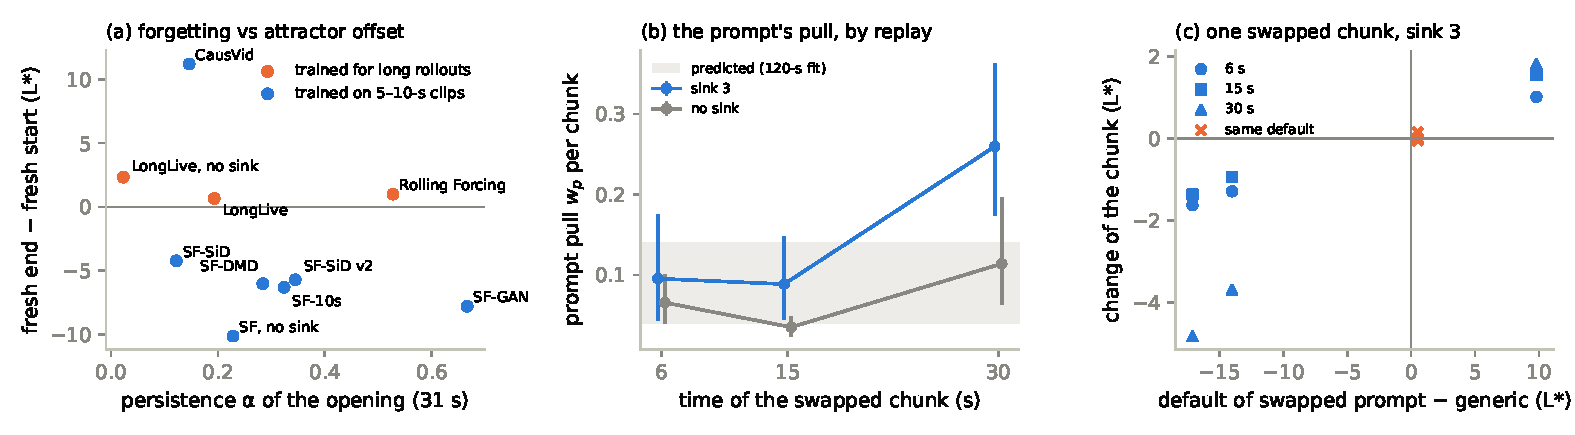
\includegraphics[width=\linewidth]{fig_mech.pdf}
\caption{(a) Two components of drift: persistence of the opening (study 6) against the attractor offset of fresh
rollouts (end minus start brightness, 4 seeds); models trained on their own long rollouts have almost no offset but
still forget. (b) The prompt's per-chunk pull measured by bit-exact replay (study 14; 16 seeds; 95\% CIs): one chunk
regenerated from identical cache, noise and random state with only the text conditioning swapped; grey: the value
implied by the recursion fitted to 120-s curves, preregistered for 15\,s. (c) The swapped chunk's change against the
difference of the prompts' defaults; a prompt with the same default has no effect.}
\label{fig:mech}
\end{figure}
Model a chunk's mean statistic as $x_{k+1} = w_w\,\bar x_{\text{window}} + w_s\,x_{\text{sink}} + w_p\,\mu$ with
$w_w + w_s + w_p = 1$, where the opening counts as a window chunk until it rolls out and $\mu$ is the prompt's default.
Without a sink the opening is eventually forgotten; with one, $\alpha_\infty = w_s/(w_s+w_p)$, so a small sink weight
keeps a large share if the prompt's pull is also small. Fitted to 120-s curves, the recursion gives $w_s = 0.060$
\ci{0.021}{0.097} and $w_w = 0.86$, implying $w_p\approx0.08$, which we preregistered as the expected value of the
replay measurement (the preregistered test was $w_p>0$). Study 14 measured 0.088 \ci{0.045}{0.149} at 15\,s. With a
sink the prompt's pull rises to 0.26 \ci{0.17}{0.36} at 30\,s (preregistered test of time invariance, $+0.16$
\ci{0.10}{0.24}), so the recursion holds for about 20\,s.
Bit-exact replay of the key--value cache measures the recursion's weights directly, by regenerating one chunk from
identical noise after changing only the sink, the window or the text conditioning: $w_s = 0.053$ \ci{0.040}{0.066} for
synthetic tone shifts (0.036 in a dose--response design), and $w_w = 0.76$ (synthetic) to 0.90--0.99 (natural
differences), in 10 development prompts $\times$ 2 seeds. The prompt's pull measured in study 14 is proportional to the
difference between the two prompts' defaults, and a prompt with the same default has no effect (Fig.~\ref{fig:mech}b,
c). The three weights sum to 1.00 with the fitted $w_w$, but to 0.90 or 1.13 with the replay-measured ones, and
$\alpha_\infty$ is 0.29--0.41 depending on which $w_s$ is used. Without a sink the measured pull is smaller (0.035 at
15\,s), so $w_p$ is not a property of the prompt alone, and fitted weights depend on the horizon. Re-rotated sinks of three or
six frames keep 0.16--0.23, below what the recursion implies; a sink at its absolute positions keeps 0.61, above it.

\section{Models outside the Wan cache family}\label{app:other}
\begin{figure}[h]
\centering
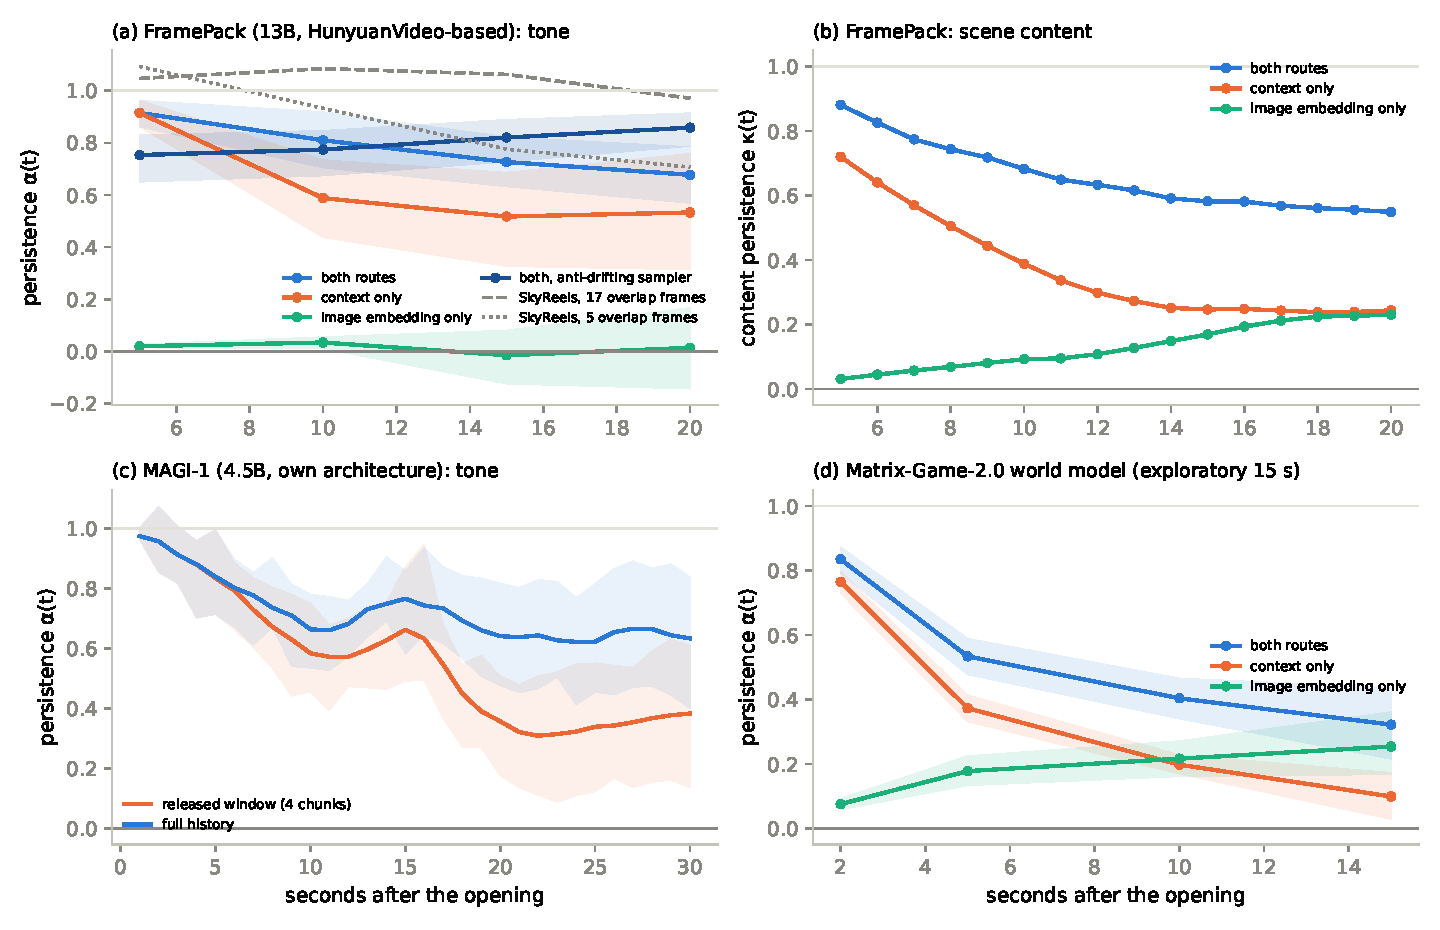
\includegraphics[width=\linewidth]{fig_framepack.pdf}
\caption{(a) FramePack (study 11, 12 scenes): the opening's brightness shift sent through both routes, only the clean
context prefix, or only the SigLIP image embedding; the anti-drifting sampler; SkyReels-V2 with 17 and 5 overlapping
frames for reference. (b) FramePack, scene content (study 17, 24 openings, city prompt): with a city frame in the
context, the opening's embedding alone pulls the video toward the opening's class. (c) MAGI-1 (study 18, 12 scenes):
the released window of four 1-s chunks against full history (1-s windows, 3-s moving average). (d) Matrix-Game-2.0, an
action-conditioned world model without text (study 15, exploratory 15-s analysis, 20 scenes): the context latent
leaves the window and is forgotten, while the rollout drifts toward the CLIP-embedded opening. Bands:
scene-bootstrap 95\% CIs.}
\label{fig:framepack}
\end{figure}

\paragraph{Matrix-Game-2.0.} The preregistered tests of study 15 used 7 scenes, as the model often collapses to black:
the context-only shift fades ($-0.24$ \ci{-0.35}{-0.14} from 5 to 30\,s), and the embedding-only shift keeps 0.43
\ci{0.13}{0.71} at 30\,s (Holm $p=0.075$, not supported); over 20 scenes at 15\,s it keeps 0.25 \ci{0.17}{0.36}
(exploratory; Fig.~\ref{fig:framepack}d).

\section{The default and the forecast}\label{app:default}
\begin{figure}[h]
\centering
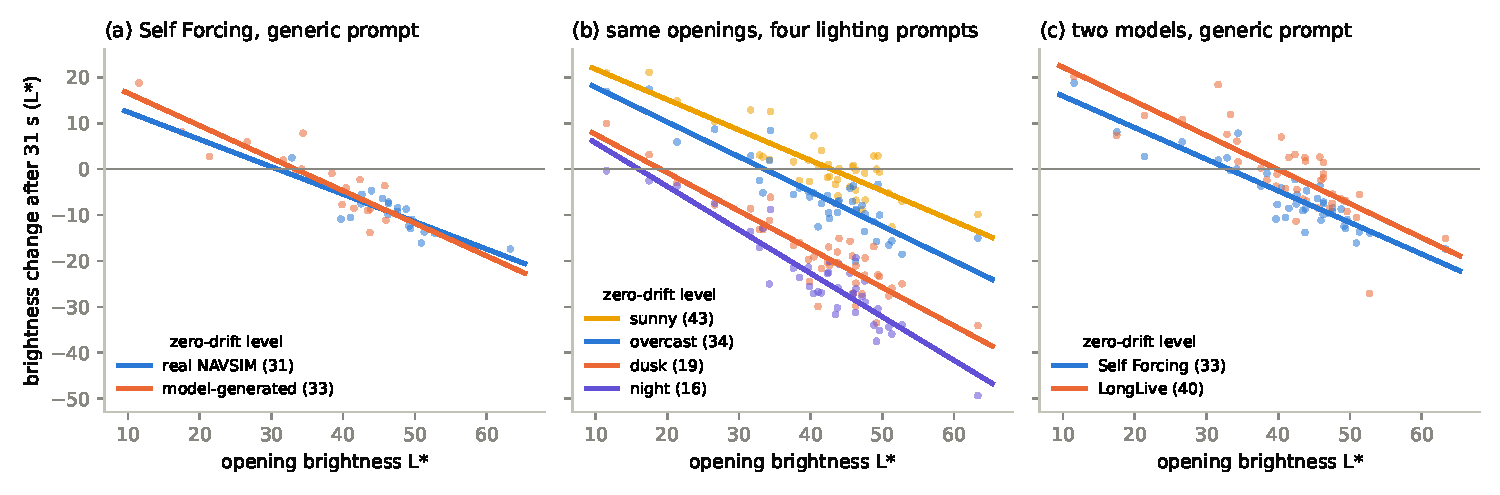
\includegraphics[width=\linewidth]{fig_default.pdf}
\caption{Brightness change after 31\,s against the opening's brightness (one dot per opening, generic or lighting prompt): (a) real and generated openings follow one line; (b) four lighting prompts set four defaults (Self Forcing); (c) two models: similar slopes, different defaults.}
\label{fig:default}
\end{figure}

\paragraph{How well does the law forecast?} Taking $\alpha$ and the generic default from the relaxation study and the
lighting defaults from the lighting experiment (different scenes and openings), $\Delta L \approx
(1-\alpha)(\mu-L_{\text{open}})$ predicts the 31-s brightness change of each opening in the calibrated-lighting study
with $r=0.82$ (Self Forcing) and $0.77$ (LongLive), mean absolute error 3.8~\Lstar. Most of this correlation reflects
the opening's brightness. The forecast of the \emph{benefit} of calibration per opening is weaker ($r=0.46$ and $0.58$),
and its mean is overpredicted ($-4.5$ predicted vs $-3.2$ and $-2.8$ observed~\Lstar). The law is a first-order guide
to a prompt choice, not a precise forecast.

%=====================================================================================================================
\section{Pitfalls for evaluating long-video models}\label{app:pitfalls}
\begin{enumerate}
\item \textbf{The GPU architecture changes the video.} With bf16, outputs are bit-identical within an architecture and
differ across A40, A100/A800 and L40S/RTX~6000 Ada. Paired designs must pin or guard the architecture.
\item \textbf{Resumed jobs can silently break pairing.} Generators that skip existing outputs resume a preempted job
wherever it lands.
\item \textbf{Image-quality scores miss drift.} MUSIQ, used by VBench for imaging quality, varies only between 66 and 69
across context strategies whose colour drift differs threefold.
\item \textbf{Natural variation is too small to estimate persistence.} Within a prompt, seeds start only about 2~\Lstar{}
apart, so within-prompt slopes of end on start brightness have intervals of about $\pm0.4$; controlled shifts are needed.
\item \textbf{Change-on-baseline regressions mislead.} Regressing change on a baseline measured with error produces
spurious regression to the mean~\cite{oldham,barnett}. Held openings are measured almost without error, and the
interventional design removes the issue.
\end{enumerate}

%=====================================================================================================================
\section{Context strategies (study 1)}\label{app:ctx}
A preregistered factorial study of 10 window and sink strategies on Self Forcing (40 prompts $\times$ 4 seeds, 31\,s)
found that a 3-frame sink cuts colour drift $D$ by 7.56 \ci{6.81}{8.32} and DINOv2 drift $K$ by 0.90; that window size
matters only without a sink; and that re-rotating the sink's positions (which keeps the query--sink distance within the range seen in training) does
not reduce $D$ ($-0.03$ \ci{-0.79}{0.72}) and increases $K$ ($+0.36$). Darkening persists with a sink (last-2-s $z_L =
-1.99$). $D$ and $K$ rise roughly linearly over 31\,s under every strategy, without a visible plateau.
